\chapter{Estado del arte}
\label{cha:state_of_art}

En este capítulo se realiza el estudio del estado del arte del presente trabajo.

\section{Tecnologías de contenedores}

Las tecnologías de contenedores se inspiran en el diseño orientado a servicios de aplicaciones. Éstas se dividen en componentes funcionales o microservicios empaquetados individualmente, junto con todas sus dependencias.

Las aplicaciones orientadas a servicios dividen la funcionalidad del sistema en contenedores que se comunican unos con otros a través de interfaces bien definidas. No tienen que preocuparse de las especificaciones del sistema anfitrión. En su lugar, cada contenedor proporciona interfaces de programación de aplicaciones (\textit{APIs}) consistentes que los clientes puedan usar para acceder al servicio. Estas estrategias permiten intercambiar o actualizar cada componente mientras la \textit{API} lo mantenga. Además, cada contenedor puede escalar o crecer de forma independiente.

Algunos de los beneficios del uso de estas tecnologías son:
\begin{itemize}
\item Abstracción del sistema anfitrión donde se ejecutará la aplicación basada en contenedores mediante interfaces definidas, con independencia de los recursos o arquitecturas del sistema anfitrión.
\item Escalabilidad en pruebas y puesta en producción.
\item Administración simplificada de dependencias y versiones de aplicaciones.
\item Ambientes de ejecución aislados a nivel de proceso.
\item Compartir contenedores evitando la duplicación y ocupando menor espacio en disco.
\end{itemize}

Dos de las destacadas tecnologías de contenedores son Docker\cite{docker}, que será la escogida y detallada en el punto \ref{docker}, y rkt\cite{rkt}. Este último es un software de código abierto del equipo que desarrolla CoreOS\cite{masteringcoreos}. Se trata de un gestor de contenedores de última generación para clústeres de Linux que descubre, verifica, extrae y ejecuta contenedores aislados de aplicaciones que pueden ser conectables. La interfaz principal de rkt comprende un solo ejecutable, en lugar de un demonio. Este diseño es aprovechado para integrarse con los sistemas de inicio existentes y con entornos de orquestación de clúster avanzados.

\begin{figure}[H]
\centering

\includegraphics[width=0.13\textwidth]{images/figures/rkt.png}
\caption{Tecnología de contenedores rkt.\footnotemark}
\end{figure}

\footnotetext{GitHub rkt. (2017). RKT logo vector [Figura]. Recuperado de \url{https://github.com/rkt/rkt/blob/master/logos/rkt-horizontal-color.png}}

\subsection{Docker}\label{docker}

En este trabajo aplicará Docker como tecnología de contenedores. Docker es un software de código abierto que proporciona las herramientas necesarias para crear y administrar contenedores ligeros y portables, automatizando el despliegue de aplicaciones. Surgió como un proyecto interno de la empresa dotCloud, por Salomón Hykes, y pasó a código abierto en marzo de 2013.

\begin{figure}[H]
\centering

\includegraphics[width=0.25\textwidth]{images/figures/docker.png}
\caption{Docker.\footnotemark}
\end{figure}

\footnotetext{Docker. (2017). Brand Guidelines [Figura]. Recuperado de \url{https://www.docker.com/brand-guidelines}}

La arquitectura de Docker se corresponde con la Figura \ref{fig:docker}. 

\begin{figure}[H]
\centering
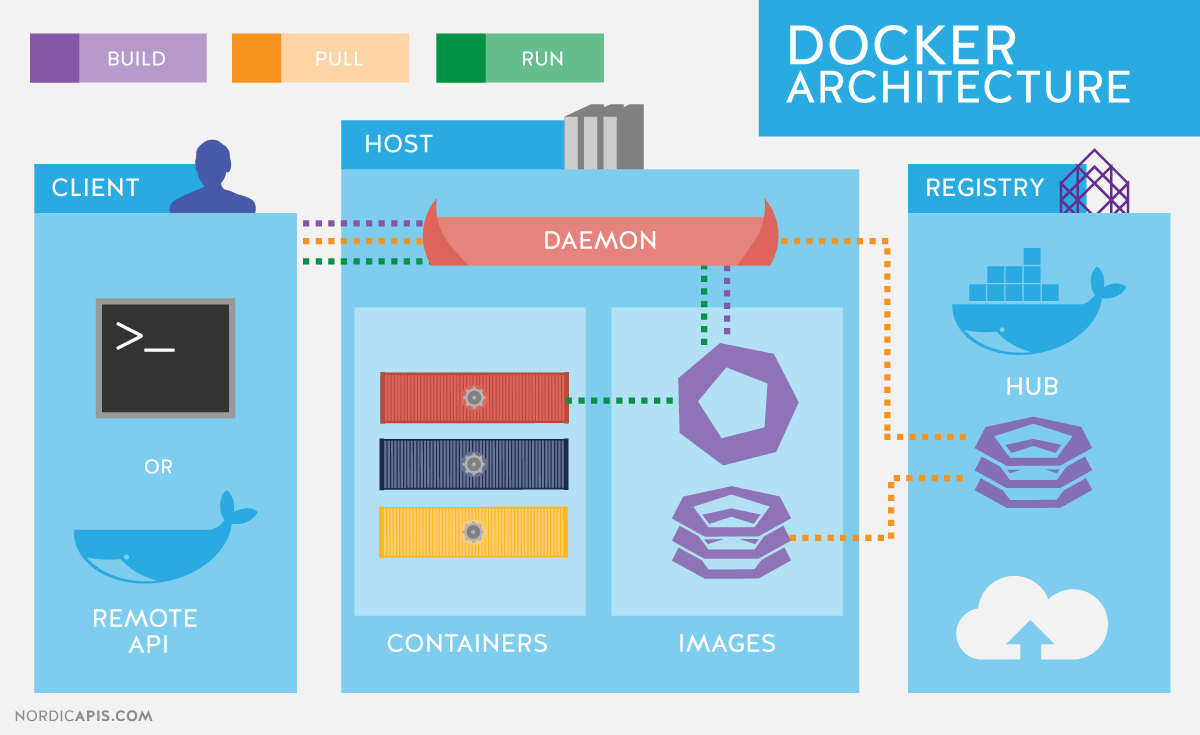
\includegraphics[width=0.6\textwidth]{images/figures/dockerarchitecture.png}
\caption{Arquitectura Docker.\footnotemark \label{fig:docker}}
\end{figure}

Docker Hub\cite{dockerhub} es un servicio de registro basado en la nube que contiene repositorios con imágenes Docker, que pueden ser públicas o privadas. Éstas son plantillas de solo lectura que consisten en una instantánea de una distribución Linux y un conjunto de aplicaciones.

Los pasos de configuración se especifican en un fichero de compilación, llamado \kode{Dockerfile}, que describe cómo crear la imagen del contenedor.


\footnotetext{Mersch. (2017). API-Driven DevOps: Spotlight on Docker [Figura]. Recuperado de \url{http://nordicapis.com/api-driven-devops-spotlight-on-docker}}

Cada instalación de Docker incluye un cliente, una \textit{API} remota y un demonio Docker. Tanto el cliente como el demonio pueden compartir un único sistema anfitrión o el demonio puede ejecutarse en un sistema anfitrión remoto. Así, los contenedores Docker contienen todo lo necesario para que la aplicación se ejecute de forma aislada, incluyendo el sistema operativo y un sistema de ficheros. Esto permite que los contenedores puedan moverse de sistema anfitrión sin riesgo de errores de configuración.

\subsection{Contenedores y Máquinas Virtuales}

Los contenedores se diferencian de las máquinas virtuales en la ubicación de la capa de virtualización y en la forma en que utilizan los recursos del sistema operativo. Esto se puede observar en la Figura \ref{fig:containervsmv}.

\begin{figure}[H]
\centering
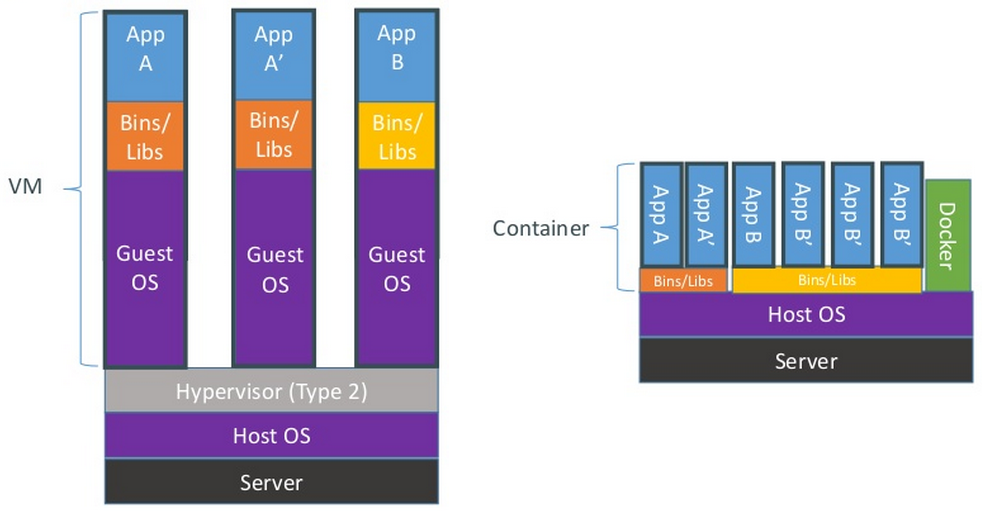
\includegraphics[width=0.6\textwidth]{images/figures/containervsmv.png}
\caption{Diferencia entre máquina virtual y contenedor.\footnotemark \label{fig:containervsmv}}
\end{figure}

Las máquinas virtuales se basan en un hipervisor que se instala sobre el hardware del sistema o del sistema operativo. Luego, las instancias de las máquinas virtuales se pueden aprovisionar a partir de los recursos disponibles en el sistema. Las máquinas virtuales están completamente aisladas unas de otras y se pueden migrar de un sistema virtualizado a otro sin tener en cuenta el hardware del sistema o los sistemas operativos.

El entorno de los contenedores está dispuesto de manera diferente. Los contenedores se instalan encima de un sistema operativo anfitrión. Éstos se pueden aprovisionar a partir de los recursos disponibles del sistema y se pueden implementar las aplicaciones necesarias. De esta manera cada aplicación contenedora comparte el mismo sistema operativo subyacente.

Los contenedores se consideran más eficientes que las máquinas virtuales desde el punto de vista de los recursos, puesto que no añaden recursos adicionales para cada sistema operativo. Las instancias resultantes son más pequeñas y más rápidas en su creación o migración y un único sistema puede albergar muchos más contenedores que máquinas virtuales.

Sin embargo, hay que tener en cuenta que el sistema operativo único presenta un único punto de error para todos los contenedores que lo utilizan. Por ejemplo, un ataque o bloqueo de \textit{malware} del sistema operativo anfitrión puede inhabilitar o afectar a todos los contenedores. Además, aunque los contenedores son fáciles de migrar, éstos sólo se pueden migrar a otros servidores con núcleos de sistema operativo compatibles.

\footnotetext{Zagur. (2016). Introducción a Docker [Parte 0] [Figura]. Recuperado de \url{http://portallinux.es/introduccion-docker-parte-0}}

\section{Sistemas operativos orientados a contenedores}

Tras el éxito y popularidad de las tecnologías de contenerización han surgido sistemas operativos modernos diseñados para funcionar de manera óptima con un ecosistema de contenedores. Estos sistemas operativos proporcionan la mínima funcionalidad requerida para implementar aplicaciones, junto con propiedades de actualización y restablecimiento.

Los sistemas operativos orientados a contenedores han evolucionado el modelo operativo tradicional moviéndose hacia el despliegue de aplicaciones dentro de contenedores, frente a la implementación de aplicaciones en la capa de aplicación. Aquí las aplicaciones son binarios autónomos que se pueden mover en su entorno de contenedor. Esta tecnología también se conoce como la virtualización del sistema operativo en el que su núcleo permite la existencia de múltiples instancias o contenedores de espacio de usuario aisladas, en lugar de una sola.

En el desarrollo de este trabajo se utilizará el sistema operativo orientado a contenedores CoreOS, descrito en el punto \ref{CoreOS}.

\subsection{CoreOS}\label{CoreOS}

CoreOS es un sistema operativo ligero de código abierto, de la compañía con el mismo nombre, basado en el núcleo de Linux y lanzado en octubre de 2013. CoreOS proporciona las características necesarias para ejecutar contenedores con un enfoque práctico para las actualizaciones del sistema operativo.

\begin{figure}[H]
\centering

\includegraphics[width=0.25\textwidth]{images/figures/coreos.png}
\caption{CoreOS.\footnotemark}
\end{figure}

\footnotetext{CoreOS. (2017). About CoreOS, Inc [Figura]. Recuperado de \url{https://coreos.com/about}}

CoreOS está diseñado para implementar una aplicación distribuida en un clúster de nodos. Así, se encarga de proporcionar la infraestructura necesaria para los despliegues en clúster, automatización, seguridad, fiabilidad y escalabilidad. CoreOS ofrece las funcionalidades mínimas necesarias para la implementación de aplicaciones dentro de contenedores de software, junto con mecanismos incorporados para el descubrimiento de servicios y el intercambio de configuración.

Los principales componentes que conforman la arquitectura de CoreOS, presente en la Figura \ref{fig:CoreOSarchitecture}, son su núcleo, systemd\cite{coreossystemd}, etcd\cite{etcd}, fleet\cite{fleet} y flannel\cite{flannel}.

\begin{figure}[H]
\centering
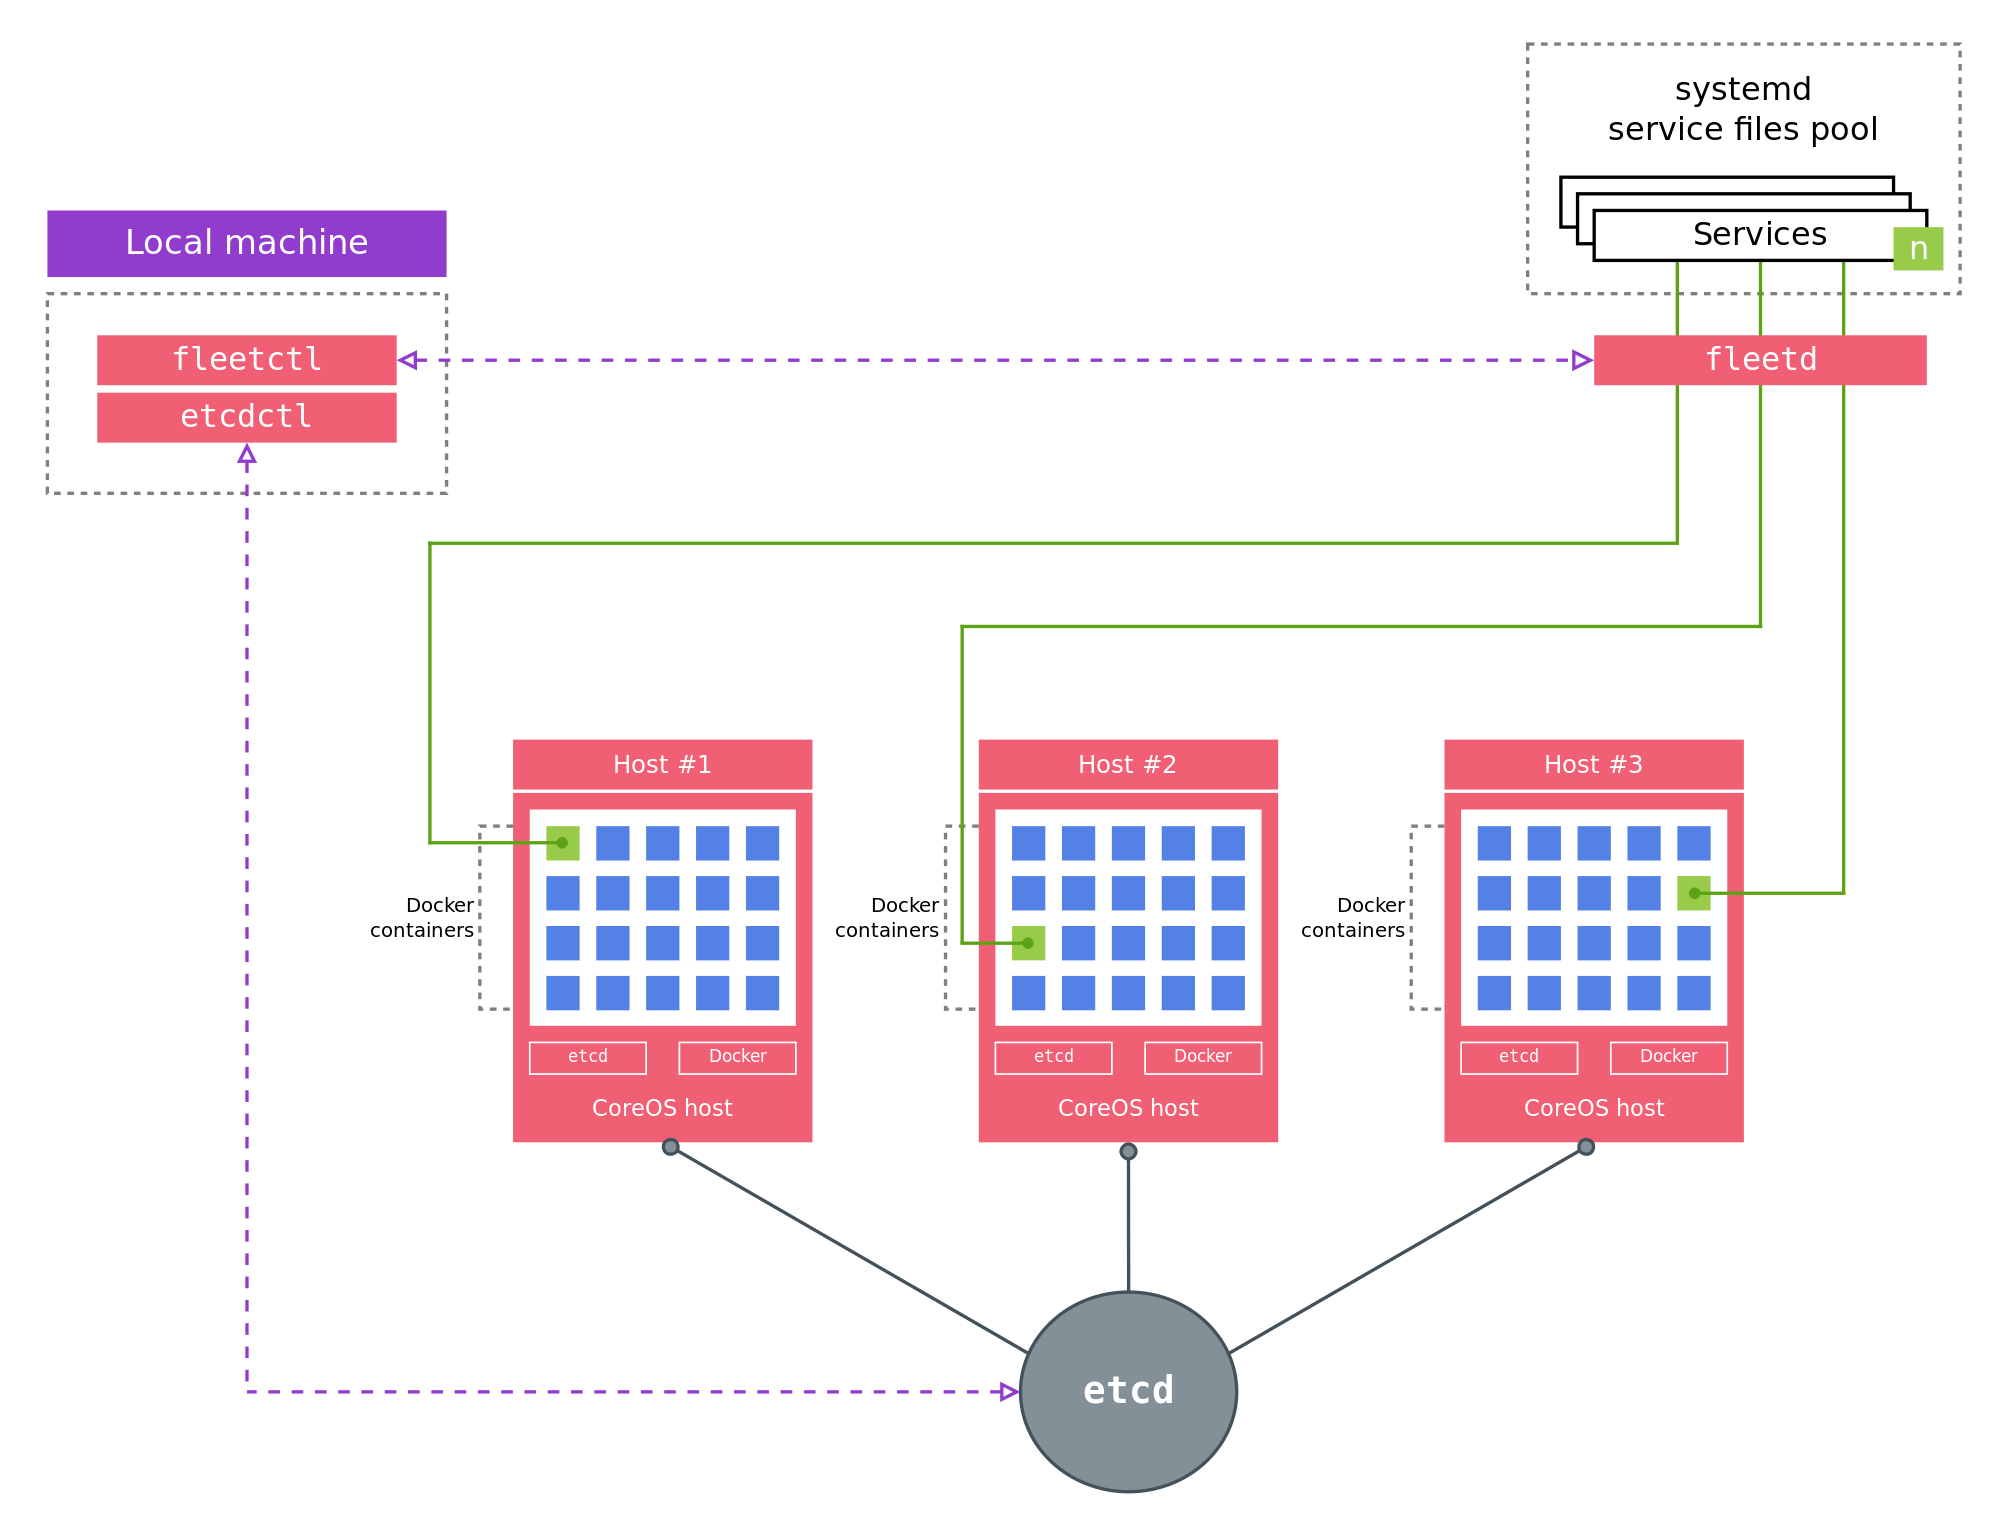
\includegraphics[width=0.8\textwidth]{images/figures/coreosarchitecture.png}
\caption{Arquitectura CoreOS.\footnotemark \label{fig:CoreOSarchitecture}}
\end{figure}

\footnotetext{Wikimedia Commons. (2015). A high-level illustration of the CoreOS cluster architecture [Figura]. Recuperado de \url{https://commons.wikimedia.org/wiki/File:CoreOS_Architecture_Diagram.svg}}

CoreOS no proporciona un gestor de paquetes, por lo que requiere que todas las aplicaciones se ejecuten dentro de sus contenedores. Para ello utiliza Docker y contenedores Linux subyacentes de virtualización para la ejecución de múltiples sistemas Linux aislados en un único sistema anfitrión de control, que sería la instancia CoreOS. De esa manera, la partición de recursos se lleva a cabo a través de múltiples instancias de espacios de usuario aisladas, en lugar de utilizar un hipervisor y una máquina virtual.

A continuación se detallan los microservicios de CoreOS a utilizar en el desarrollo de este trabajo.

\subsubsection{Systemd}

Systemd es un sistema de inicio que CoreOS utiliza para iniciar, detener y administrar procesos. Como sistema de inicio tiene las funciones de ser el primer proceso en comenzar, controlar el orden y ejecución de todos los procesos de usuario, ocuparse de reiniciarlos si mueren o cuelgan y de sus propiedadades y recursos. Si el servicio systemd se cancela, todos los procesos asociados con el servicio, incluidos los bifurcados, se eliminan. 

Las unidades systemd se ejecutan y controlan una sola máquina. Éstas describen una tarea en particular junto con sus dependencias y orden de ejecución. Algunas unidades se inician en el sistema de forma predeterminada y otras por usuarios.

La interfaz de línea de comandos (\textit{CLI}) systemctl puede utilizarse para controlar las unidades systemd. Éstas pueden ser creadas a partir de una plantilla y utilizarla para instanciar varias unidades.

Algunos tipos de unidad systemd son \textit{service} y \textit{socket}. El tipo más común es \textit{service} y se utiliza para definir un servicio con sus dependencias. El tipo \textit{socket} se utiliza para exponer los servicios al mundo externo. Por ejemplo, \textit{docker.service} expone la conectividad externa al motor Docker a través de \textit{docker.socket}. Los \textit{sockets} también se pueden utilizar para exportar registros a máquinas externas.

\subsubsection{Etcd}

Etcd es un sistema de almacenamiento distribuido de pares clave-valor utilizado por todas las máquinas del clúster CoreOS para leer, escribir e intercambiar datos. Además, se utiliza para compartir la configuración y los datos de monitorización en los equipos CoreOS y para realizar el descubrimiento del servicio. Los demás servicios de CoreOS usan etcd como una base de datos distribuida. 

La utilidad etcdctl es la interfaz \textit{CLI} para etcd.

Los parámetros de configuración de etcd se pueden usar para modificar propiedades de un sólo miembro etcd o de todo el clúster. Estas opciones son:

\begin{itemize}
\item Miembro: Nombre, directorio de datos e intervalo de latido.
\item Clúster: Señal de descubrimiento y nodos de clúster iniciales.
\item Proxy: Activado/Desactivado e intervalos.
\item Seguridad: Certificado y clave.
\item Registro: Habilitar/Deshabilitar registro y niveles de registro.
\end{itemize}

Las operaciones principales que se pueden hacer usando etcd son:

\begin{itemize}
\item Establecer, obtener y eliminar operaciones de un par clave-valor.
\item Establecer una clave que expire automáticamente tras un tiempo definido. 
\item Establecer una clave basada en la comprobación de una condición.
\item Claves ocultas.
\item Observación y espera ante cambios en claves.
\item Creación de claves bajo petición.
\end{itemize}

\subsubsection{Fleet} \label{fleet}

El servicio fleet es un gestor o planificador que controla la creación de servicios a nivel de clúster. Mientras que systemd actúa como sistema de inicio para un nodo, fleet es el sistema de inicio para el clúster y usa el servicio etcd para la comunicación entre nodos.

Al tratarse de una herramienta para la orquestación de contenedores será descrita con mayor detalle en el punto \ref{sec:herramientas}.

\subsubsection{Flannel}

Flannel utiliza una red de superposición para permitir que contenedores, a través de diferentes anfitriones, se comuniquen entre sí.

Entre sus características cabe destacar que flannel se ejecuta sin un servidor central y utiliza etcd para la comunicación entre los nodos.

Cada nodo del clúster solicita un rango de direcciones IP para los contenedores creados en ese anfitrión y lo registra con etcd. Como cada nodo del clúster conoce el rango de direcciones IP asignado para cada otro nodo, sabe cómo llegar a los contenedores creados en cualquier nodo del clúster. Cuando se crean contenedores, los contenedores obtienen una dirección IP dentro del rango asignado al nodo y si necesitan comunicarse a través de anfitriones, flannel hace la encapsulación basada en el protocolo elegido. Así, en el nodo destino desencapsula el paquete y lo entrega al contenedor.

Las razones por las que se necesita crear redes de contenedores son:
\begin{itemize}
\item Los contenedores necesitan comunicarse con el mundo exterior.
\item Los contenedores deben ser accesibles desde el mundo exterior para que éste pueda utilizar los servicios que proporcionan.
\item Los contenedores necesitan comunicarse con la máquina anfitriona.
\item Debería haber conectividad entre contenedores en el mismo anfitrión y entre anfitriones.
\end{itemize}

\subsubsection{Confd}

La herramienta confd está diseñada para ver cambios en los almacenes distribuidos de clave-valor. Se ejecuta dentro de un contenedor Docker y se utiliza para activar modificaciones de configuración y recargas de servicio.

Esta herramienta de gestión de configuración está construida en la parte superior de etcd. Así, confd puede ver ciertas claves en etcd y actualizar los archivos de configuración relacionados a ellas tan pronto como cambie. Luego, confd puede volver a cargar o reiniciar las aplicaciones relacionadas con los archivos de configuración actualizados. Esto permite automatizar los cambios de configuración en todos los servidores del clúster y asegura que todos los servicios están siempre buscando la última configuración.

\subsection{Otros}

Otros sistemas operativos orientados a contenedores son Red Hat Enterprise Linux (RHEL) Project Atomic\cite{rhel7} y Snappy Ubuntu Core\cite{ubuntucore}.

Project Atomic, lanzado en 2014, facilita la arquitectura centrada en la aplicación proporcionando una solución para desplegar aplicaciones basadas en contenedores de forma rápida y confiable. La actualización atómica y la reversión de aplicaciones y anfitriones permiten la implementación de pequeñas mejoras frecuentes.

\begin{figure}[H]
\centering

\includegraphics[width=0.1\textwidth]{images/figures/projectatomic.png}
\caption{Project Atomic.\footnotemark}
\end{figure}

\footnotetext{GitHub Project Atomic. (2017). Project Atomic [Figura]. Recuperado de \url{https://github.com/projectatomic}}

Por su parte Snappy Ubuntu Core, lanzado en 2014, es un sistema operativo que usa una imagen de servidor mínima con las mismas bibliotecas que el sistema operativo Ubuntu actual. Su enfoque ágil es más rápido, más fiable y permite ofrecer mayores garantías de seguridad para aplicaciones y usuarios. Las aplicaciones se pueden actualizar de forma atómica y revertirse si es necesario, pensando en contenedores.

\begin{figure}[H]
\centering

\includegraphics[width=0.15\textwidth]{images/figures/ubuntucore.jpg}
\caption{Ubuntu Core.\footnotemark}
\end{figure}

\footnotetext{(2016). Ubuntu Core 16 delivers foundation for secure IoT [Figura]. Recuperado de \url{https://insights.ubuntu.com/2016/11/03/ubuntu-core-16-delivers-foundation-for-secure-iot}}

\section{Herramientas para la orquestación de contenedores} \label{sec:herramientas}

Un sistema de orquestación de contenedores trata el hardware dispar de la infraestructura como una colección y lo representa para la aplicación como un único recurso. También, programa los contenedores basándose en las restricciones de los usuarios y utiliza la infraestructura de la manera más eficiente posible, escalando los contenedores dinámicamente y manteniendo los servicios en alta disponibilidad.

La herramienta para la orquestación de contenedores usada en el presente trabajo es Fleet, descrita en el punto \ref{Fleet}.

\subsection{Fleet}\label{Fleet}

Como se comentó en el punto \ref{fleet}, fleet es un componente de CoreOS que controla la creación de servicios a nivel de clúster.

Fleet utiliza el modelo maestro-esclavo, donde el motor fleet desempeña el papel de maestro y el agente fleet representa el papel de esclavo. El motor es reponsable de programar las unidades fleet y el agente de ejecutarlas y divulgar su estado al motor. Las unidades fleet también constan de metadatos para controlar dónde se ejecuta la unidad con respecto a la propiedad del nodo, así como la base de otros servicios que se ejecutan en ese nodo en particular. El agente procesa la unidad y la ofrece a systemd para su ejecución. Si un nodo muere se elige un nuevo motor y las unidades de programa en ese nodo se reprograman en un nuevo nodo. Systemd proporciona alta disponibilidad a nivel de nodo, mientras que fleet lo hace a nivel de clúster. Así, fleet se utiliza principalmente para la orquestación de servicios críticos del sistema, usando systemd.

Los metadatos se pueden utilizar en archivos de servicio fleet para controlar la programación y las opciones X-Fleet se usan para especificar restricciones al programar el servicio. Entre las disponibles se encuentran:
\begin{itemize}
\item \textit{MachineMetaData}: El servicio se programa basado en metadatos coincidentes.
\item \textit{Global}: El mismo servicio se programa en todos los nodos del clúster.
\end{itemize}

\subsection{Otras}\label{Otras}

Otras herramientas para la orquestación de contenedores en la actualidad son Kubernetes\cite{kubernetes}, Docker Swarm\cite{swarm} y Apache Mesos\cite{apachemesos}.

\subsubsection{Kubernetes}

Kubernetes es una plataforma de código abierto para la orquestación de contenedores, iniciada por Google.

\begin{figure}[H]
\centering

\includegraphics[width=0.25\textwidth]{images/figures/kubernetes.png}
\caption{Kubernetes.\footnotemark}
\end{figure}

\footnotetext{(2017). Kubernetes logo [Figura]. Recuperado de \url{https://opencredo.com/kubernetes}}

La unidad más pequeña en Kubernetes es un \textit{pod}. Los \textit{pods} son un conjunto de contenedores que se encuentran juntos en un único nodo. Cada \textit{pod} tiene una dirección IP y todos los contenedores de ese \textit{pod} la comparten. Kubernetes sigue la arquitectura maestro-esclavo.

Como se muestra en la Figura \ref{fig:kubernetesarchitecture}, Kubernetes se compone de múltiples servicios. Kubelet es responsable del estado de ejecución de cada nodo. Se ocupa de iniciar, detener y mantener los contenedores de aplicaciones. Kube-proxy se ocupa de la redirección de servicios y el balanceo de carga del tráfico en los \textit{pods}. El servidor \textit{API} sirve a la \textit{API} estándar utilizando \textit{JSON} sobre \textit{HTTP}, proporcionando tanto la interfaz interna como externa a Kubernetes. Así, el servidor \textit{API} procesa y valida las peticiones \textit{REST} y actualiza el estado de los objetos \textit{API} en etcd, permitiendo a los clientes configurar cargas de trabajo y contenedores. El planificador es el componente conectable que selecciona en qué nodo debería ejecutarse un \textit{pod} no programado basado en la disponibilidad de recursos y las cargas de trabajo existentes. Por su parte, el controlador de replicación es necesario para mantener la alta disponibilidad de \textit{pods} y crear varias instancias. 

\begin{figure}[H]
\centering
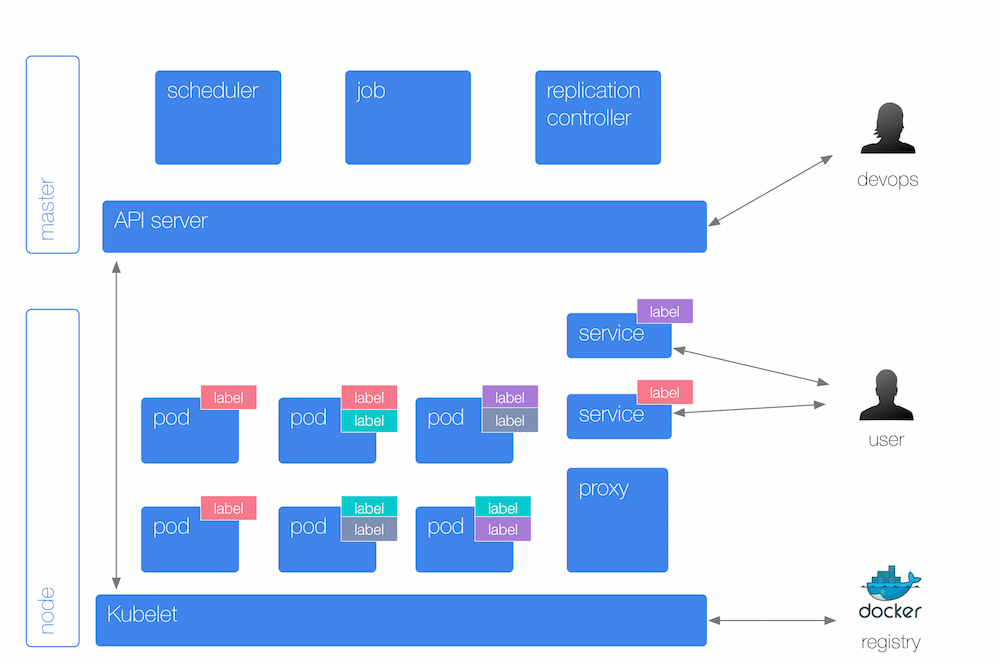
\includegraphics[width=0.6\textwidth]{images/figures/kubernetesarchitecture.png}
\caption{Arquitectura Kubernetes.\footnotemark \label{fig:kubernetesarchitecture}}
\end{figure}

\footnotetext{Mhausenblas. (2016). Kubernetes Community Resources [Figura]. Recuperado de \url{http://k8s.info/cs.html}}

\subsubsection{Docker Swarm}

Docker Swarm es la solución de orquestación nativa de Docker.

\begin{figure}[H]
\centering

\includegraphics[width=0.4\textwidth]{images/figures/swarm.png}
\caption{Docker Swarm.\footnotemark}
\end{figure}

\footnotetext{(2017). Swarm: a Docker-native clustering system [Figura]. Recuperado de \url{https://github.com/docker/swarm}}

Como se muestra en la Figura \ref{fig:dockermasterandagent}, con su uso se administra el clúster como entidad en lugar de administrar nodos individuales. Esta herramienta tiene un planificador integrado que decide la ubicación de los contenedores en el clúster y utiliza restricciones y afinidades específicas del usuario para decidir esa ubicación. En su arquitectura existe un maestro que se encarga de la planificación de contenedores Docker basado en el algoritmo planificador, restricciones y afinidades. Para proporcionar alta disponibilidad se pueden ejecutar múltiples maestros en paralelo, distribuyendo las cargas de trabajo uniformemente. Los agentes se ejecutan en cada nodo y se comunican con el maestro a partir del descubrimiento, necesario porque se ejecutan en diferentes nodos no iniciados por él.

\begin{figure}[H]
\centering
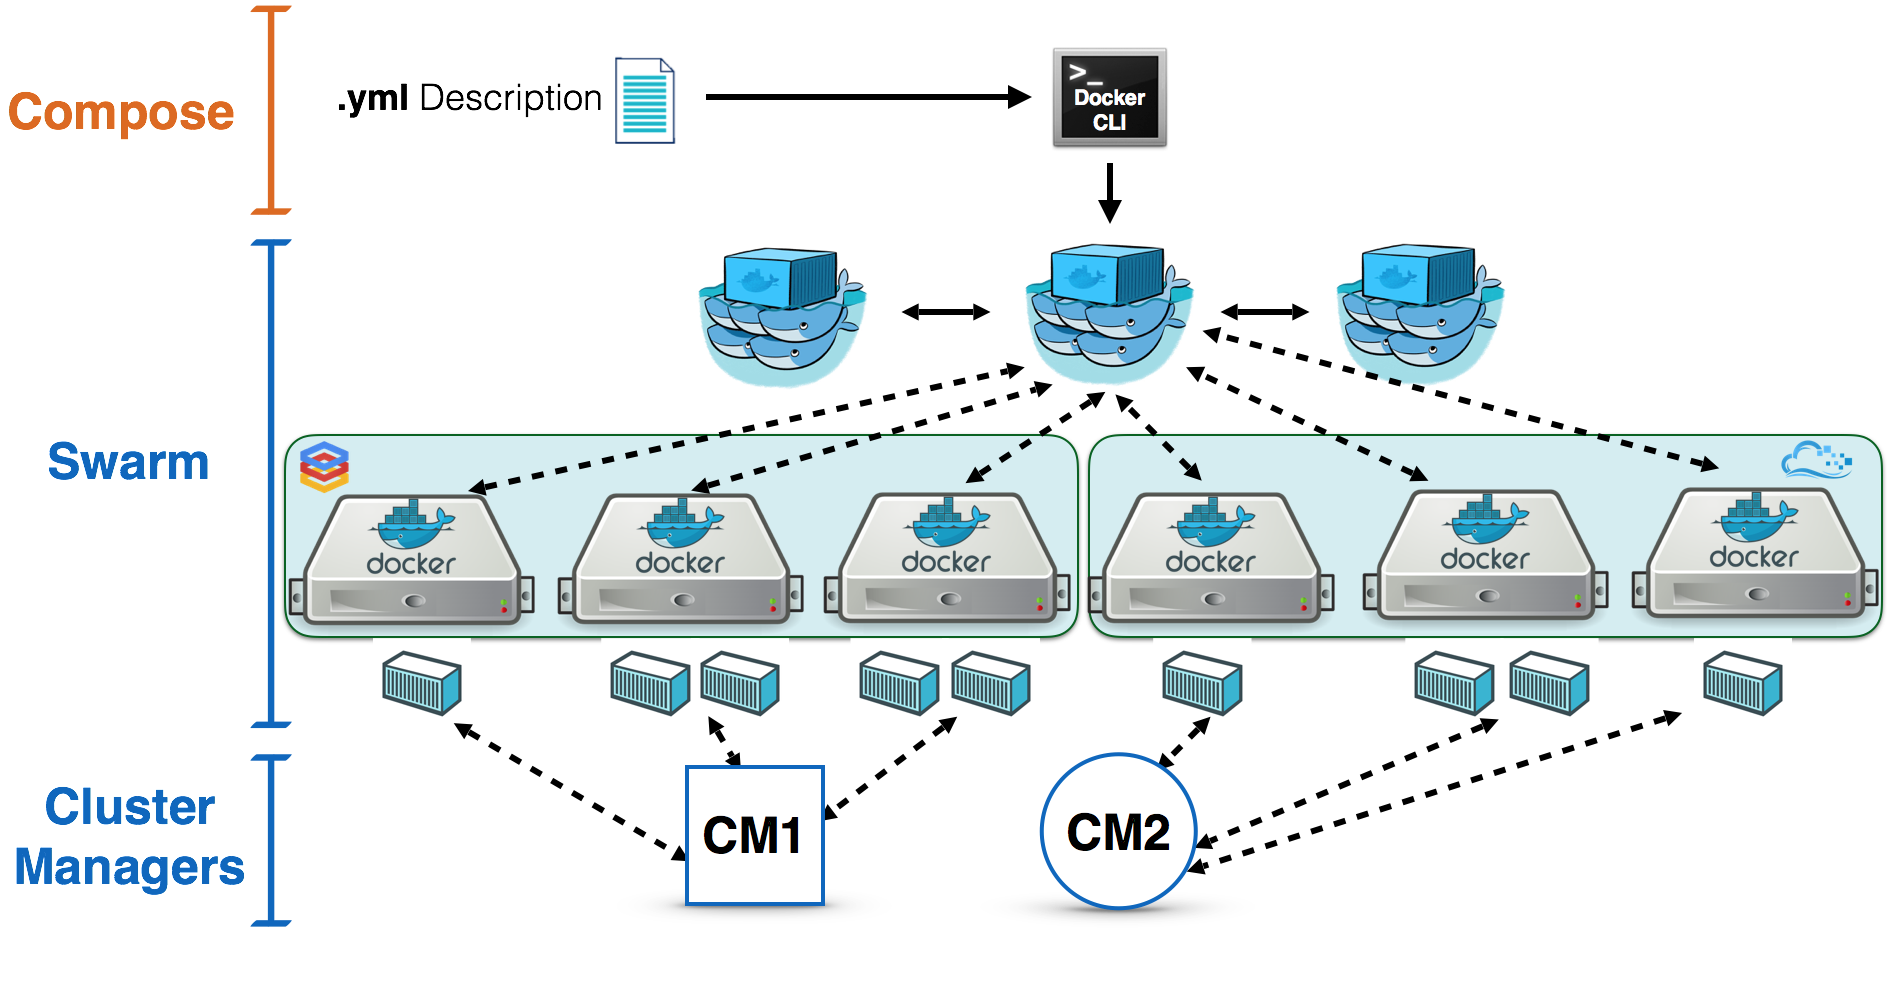
\includegraphics[width=0.65\textwidth]{images/figures/dockermasterandagent.png}
\caption{Composición de maestros y agentes en Docker Swarm.\footnotemark \label{fig:dockermasterandagent}}
\end{figure}

\footnotetext{Alba. (2015). Deploy and Manage Any Cluster Manager with Docker Swarm [Figura]. Recuperado de \url{https://blog.docker.com/2015/11/deploy-manage-cluster-docker-swarm}}
	
\subsubsection{Apache Mesos}

Apache Mesos, desarrollado en la Universidad de California Berkeley, combina el sistema operativo con el administrador de clústeres.

\begin{figure}[H]
\centering

\includegraphics[width=0.25\textwidth]{images/figures/apachemesoslogo.png}
\caption{Apache Mesos.\footnotemark}
\end{figure}

\footnotetext{(2017). OpenCredo are Experts in Apache Mesos [Figura]. Recuperado de \url{https://opencredo.com/expertise/experts-in-apache-mesos}}

Como se muestra en la Figura \ref{fig:apachemesos}, Mesos consiste en un demonio maestro que gestiona los demonios agentes que se ejecutan en cada nodo del clúster y los marcos de Mesos que ejecutan tareas en estos agentes. El maestro permite un uso compartido de recursos a través de marcos. Cada oferta de recursos contiene una lista de agentes. El maestro decide cuántos recursos ofrecer a cada marco de acuerdo con una determinada política de organización. Para soportar un conjunto diverso de políticas, el maestro emplea una arquitectura modular que facilita la adición de nuevos módulos de asignación a través de un mecanismo de complemento. Un \textit{framework} que se ejecuta en la parte superior de Mesos consta de dos componentes: un programador que se registra con el maestro y un proceso ejecutor que se ejecuta en los nodos del agente para ejecutar las tareas del marco. Mientras que el maestro determina cuántos recursos se ofrecen a cada marco, los planificadores de los marcos seleccionan cuál de los recursos ofrecidos utilizar.

\begin{figure}[H]
\centering
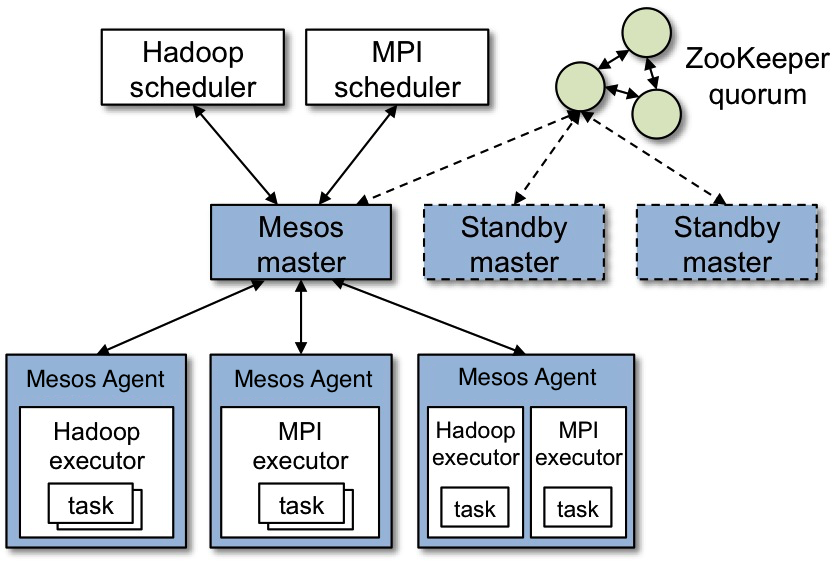
\includegraphics[width=0.45\textwidth]{images/figures/apachemesos.png}
\caption{Abstracción de nodos en Apache Mesos.\footnotemark \label{fig:apachemesos}}
\end{figure}

\footnotetext{Apache Mesos. (2017). Mesos Architecture [Figura]. Recuperado de \url{http://mesos.apache.org/documentation/latest/architecture}}

\section{Proveedores de Infraestructura como Servicio}

La Infraestructura como Servicio (\textit{IaaS}) es uno de los tres modelos fundamentales en el campo de la computación en la nube, junto con la Plataforma como Servicio (\textit{PaaS}) y el Software como Servicio (\textit{SaaS}). Se trata de una infraestructura informática inmediata que se aprovisiona y administra a través de una conexión pública, normalmente Internet.

Este modelo de servicio proporciona acceso a recursos informáticos situados en un entorno virtualizado, la nube. De esta manera permite reducir o escalar recursos  concretos con rapidez para ajustarlos a la demanda, pagando por uso y evitando el gasto y complejidad que suponen la compra y administración de una infraestructura física propia.

Existen proveedores de estos servicios informáticos en la nube que administran la infraestructura, mientras que el cliente solo tiene que configurar y administrar su propio software.

Los recursos informáticos ofrecidos consisten en hardware virtualizado o infraestructura de procesamiento. La definición de \textit{IaaS} abarca aspectos como el espacio en servidores virtuales, conexiones de red, ancho de banda, direcciones IP y balanceadores de carga. Físicamente, el repertorio de recursos hardware disponibles procede de multitud de servidores y redes, generalmente distribuidos entre numerosos centros de datos.

Entre las ventajas de \textit{IaaS} se encuentran:
\begin{itemize}
\item Eliminación del gasto en capital y corriente eléctrica.
\item Adquisición de nuevos recursos con rapidez.
\item Respuesta rápida ante cambios de demanda, aumentando y reduciendo recursos.
\item Mayor eficiencia, puesto que se garantiza que se utiliza la capacidad máxima de la infraestructura física.
\item Mayor seguridad y protección de los recursos de información.
\end{itemize}

Los ejemplos más conocidos son Amazon Web Services\cite{aws wiki} y DigitalOcean\cite{digitaloceanwiki}.

DigitalOcean, creado en 2011 por Ben y Moisey Uretsky, es un proveedor Estadounidense de servidores virtuales privados.

\begin{figure}[H]
\centering

\includegraphics[width=0.25\textwidth]{images/figures/digitalocean.png}
\caption{DigitalOcean.\footnotemark}
\end{figure}

\footnotetext{DigitalOcean (2017). Logos and badges [Figura]. Recuperado de \url{https://www.digitalocean.com/company/logos-and-badges}}

Entre sus características más destacadas está que sus servidores en la nube, llamados \textit{droplets}, pueden ser provisionados típicamente en 55 segundos. Además, provee discos duros \textit{SSD} de alto rendimiento y virtualización \textit{KVM}. En general aporta servicios mensuales por 5 dólares al mes, continuando con facturación por hora.

En la ejecución de este proyecto se aplicará el uso de Amazon Web Services como proveedor de Infraestructura como Servicio, detallado en el punto \ref{subAWS}.

\subsection{Amazon Web Services} \label{subAWS}

Amazon Web Services (AWS) es una plataforma de servicios de computación en la nube ofrecida a través de Internet por Amazon.com y lanzada en 2006.

\begin{figure}[H]
\centering

\includegraphics[width=0.17\textwidth]{images/figures/aws.png}
\caption{Amazon Web Services.\footnotemark}
\end{figure}

\footnotetext{Amazon Web Services (2017). AWS Co-Marketing Tools [Figura]. Recuperado de \url{https://aws.amazon.com/co-marketing}}

AWS está situado en distintas regiones geográficas. Cada región está totalmente contenida dentro de un solo país y todos sus datos y servicios permanecen dentro de ella. Cada una tiene múltiples zonas de disponibilidad con diferentes centros de datos que proporcionan servicios de AWS.

Este proveedor dispone de una capa gratuita diseñada para permitir obtener experiencia práctica con los servicios en la nube de AWS. Ésta incluye 12 meses a partir de la fecha de inscripción, así como ofertas de servicios adicionales que no vencen al final de este período. No obstante existen límites de uso. A partir de este primer año se empieza a pagar por horas de uso.

En la elaboración de este trabajo se utilizarán los siguientes servicios:

\subsubsection{AWS Identity and Access Management (IAM)}

AWS Identity and Access Management (IAM)\cite{iam} es un servicio web gratuito que permite controlar de forma segura el acceso a los recursos de AWS por parte de los usuarios. Facilita el acceso compartido a la cuenta AWS, concediendo permisos a otros usuarios para administrar y utilizar los recursos sin tener que compartir la clave de acceso, y la concesión de permisos diferentes a distintos usuarios para diferentes recursos.

\subsubsection{Amazon Elastic Compute Cloud (Amazon EC2)}

Amazon Elastic Compute Cloud (Amazon EC2)\cite{ec2} proporciona la capacidad de computación escalable en la nube de AWS. Permite realizar el despliegue de servidores virtuales, configurar seguridad, redes y administrar el almacenamiento. Este servicio permite escalar o reducir los requisitos bajo demanda o picos de popularidad. La principal característica es el entorno virtual de computación o instancia. Además, ofrece otras funciones como plantillas preconfiguradas, varios tipos de instancias o configuraciones, inicio de sesión seguro utilizando pares de claves, volúmenes de almacenamiento temporales, regiones y zonas de disponibilidad y grupos de seguridad.

\subsubsection{Amazon Virtual Private Cloud (Amazon VPC)}

Amazon Virtual Private Cloud (Amazon VPC)\cite{vpc} permite lanzar los servicios AWS en una red virtual definida. Una nube virtual privada (VPC) es una red virtual dedicada a la cuenta de AWS. Está aislada de otras redes virtuales en la nube AWS y permite iniciar los recursos en ella. Permite seleccionar un rango de direcciones IP, crear subredes, configurar tablas de rutas, pasarelas de red y realizar otras configuraciones de seguridad. Otro elemento a usar es la subred que es un rango de direcciones IP en la VPC. Los grupos de seguridad se utilizan para proteger los recursos de AWS en cada subred.


\section{Otras herramientas tecnológicas}

A continuación se describirán otra serie de herramientas necesarias para la elaboración de este trabajo.

\subsection{Vagrant}

Vagrant\cite{vagrant} es una herramienta de código abierto para crear y configurar entornos de desarrollo portátiles y virtualizados, centrada en la automatización.

\begin{figure}[H]
\centering

\includegraphics[width=0.1\textwidth]{images/figures/vagrant.png}
\caption{Vagrant.\footnotemark}
\end{figure}

\footnotetext{Wikipedia (2013). Vagrant (software) [Figura]. Recuperado de \url{https://es.wikipedia.org/wiki/Vagrant_(software)}}

Vagrant fue creada en enero de 2010 por Mitchell Hashimoto, que en 2012 creó la organización HashiCorp para respaldar su desarrollo a tiempo completo, contando con la contribución de una fuerte comunidad de desarrolladores. Está escrito en lenguaje Ruby pero puede ser utilizado en proyectos escritos en otros lenguajes de programación.

La idea central detrás de su creación reside en el hecho de que el mantenimiento del entorno de desarrollo se hace cada vez más difícil a medida que el proyecto crece. De esta manera, Vagrant proporciona ambientes de trabajo menos complejos de configurar, reproducibles y portátiles.

Esta herramienta utiliza aprovisionadores y proveedores como bloques de construcción para administrar los entornos de desarrollo. Los primeros son herramientas que permiten a los usuarios personalizar la configuración de entornos virtuales, mientras que los proveedores son los servicios que Vagrant utiliza para lanzar y crear los propios entornos virtuales.

Para su puesta en marcha se utiliza un fichero de configuración denominado \kode{Vagrantfile}. Su función principal es describir el tipo de máquina requerida y cómo configurarla y proveerla. Por otro lado, existen cajas que son el formato de paquetes para los ambientes Vagrant. Una caja puede ser utilizada por cualquier persona en cualquier plataforma que soporte Vagrant para crear un entorno de trabajo idéntico.

\subsection{VirtualBox}

VirtualBox\cite{vagrantboxes} es un software de virtualización de código abierto para arquitecturas \textit{x86/amd64}. 

\begin{figure}[H]
\centering

\includegraphics[width=0.1\textwidth]{images/figures/virtualbox.png}
\caption{VirtualBox.\footnotemark}
\end{figure}

\footnotetext{Wikipedia (2010). VirtualBox logo [Figura]. Recuperado de \url{https://commons.wikimedia.org/wiki/File:Virtualbox_logo.png}}

Este hipervisor de tipo II o \textit{hosted}, se caracteriza porque permite instalar sistemas operativos adicionales, conocidos como sistemas invitados o máquinas virtuales, dentro de otro sistema operativo, sistema anfitrión, cada uno con su propio ambiente virtual.

VirtualBox fue creado originalmente por la empresa alemana Innotek GmbH en enero de 2007. Actualmente es desarrollado por Oracle Corporation y existen dos versiones gratuitas. Por un lado la llamada Oracle VM VirtualBox, sujeta a la licencia de "Uso Personal y de Evaluación VirtualBox". Por otro lado, VirtualBox OSE, sujeta a la licencia GPL.

Entre sus características más importantes se destaca que es multiplataforma, en referencia a las arquitecturas soportadas; multi huéspedes, por la variedad y cantidad de sistemas operativos que puede virtualizar; y ofrece portabilidad, al poder importar y exportar las máquinas virtuales a otros sistemas.

\subsection{GitHub}

GitHub\cite{GitHub} es una plataforma de desarrollo colaborativo de software para alojar proyectos utilizando el sistema de control de versiones Git. El código se almacena de forma pública, aunque también se puede hacer de forma privada, creando una cuenta de pago.

\begin{figure}[H]
\centering

\includegraphics[width=0.12\textwidth]{images/figures/github.png}
\caption{GitHub.\footnotemark}
\end{figure}

\footnotetext{GitHub (2017). GitHub Logos and Usage [Figura]. Recuperado de \url{https://github.com/logos}}

Esta herramienta permite alojar repositorios de código y ofrece utilidades para el trabajo en equipo, dentro de un proyecto, algunas de las cuales son:
\begin{itemize}
\item Wiki: Mantenimiento de distintas versiones de páginas.
\item Sistema de seguimiento de problemas: Permite a los miembros de un equipo detallar un problema con el software o una sugerencia.
\item Visor de ramas: Permite comparar los progresos realizados en las distintas ramas del repositorio.
\end{itemize}

Además, se puede contribuir a mejorar el software de otros usuarios, a partir de la creación de programas de código abierto que fomentan el software libre.

\subsection{Travis CI}

Travis CI\cite{travisci} es una compañia y sistema distribuido que ofrece servicios de Integración y Despliegue continuos (CI/CD) gratuitos o de pago.

\begin{figure}[H]
\centering

\includegraphics[width=0.3\textwidth]{images/figures/travisci.jpg}
\caption{Travis CI.\footnotemark}
\end{figure}

\footnotetext{Travis CI (2017). Logo [Figura]. Recuperado de \url{https://travis-ci.com/logo}}

El servicio gratuito permite conectar el repositorio de GitHub público para poder regenerar el proyecto tras cada cambio. Cuando lo detecta utiliza el fichero de configuración \kode{.travis.yml} para realizar las acciones descritas en él. Este fichero contiene las precondiciones, condiciones y postcondiciones necesarias para construir y desplegar la aplicación de manera automática. Ejemplos de dichas acciones son la comprobación de los tests, construir una nueva imagen Docker y subirla al repositorio Docker Hub.

Entre los beneficios que aporta están la reducción de riesgos y tiempo, de procesos manuales repetitivos, la obtención de una versión de software mediante un proceso conocido, confiable, probado, versionado y repetible y la mejora la visibilidad del estado del proyecto. Además, mantiene la calidad de todo el sistema mediante la ejecución periódica de los tests, identificando problemas y ayudando a corregirlos antes de pasar a producción.

\subsection{Softcover}

Para la elaboración de la memoria se utiliza la gema Ruby Softcover\cite{softcover} que es un sistema de composición de libros electrónicos para autores técnicos. Depende de otra gema, polytexnic, para convertir la entrada de \textit{Markdown} o \textit{PolyTeX} a \textit{HTML} y \textit{LaTeX}, y de ahí a \textit{EPUB}, \textit{MOBI} y \textit{PDF}.


